% !TEX root = Kreisfahrt.tex
\begin{figure}
    \centering
    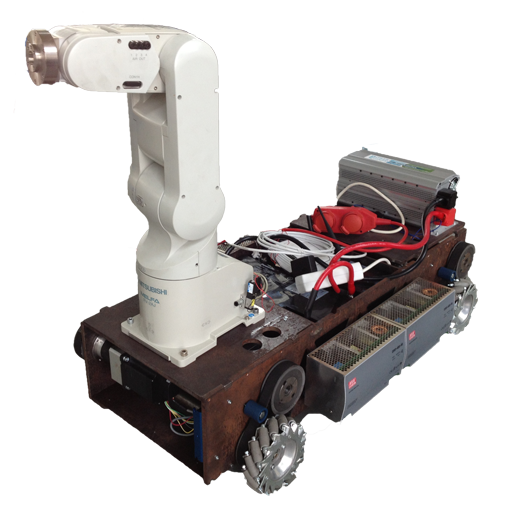
\includegraphics[width=.9\textwidth]{Abbildungen/Roboter}
    \caption{Der verwendete Roboter mit montiertem Knickarm}
\end{figure}
\newpage

\section{Einleitung}
Der Mecanum-Roboter ist ein omnidirektionales Fahrzeug. Er kann ohne Lenkung aus jeder Position in eine beliebige Richtung fahren. Grund dafür sind die verwendeten Allseitenräder -- Mecanum-Räder -- auf deren Umlauffläche 15 weitere tonnenförmige Hilfsräder angebracht sind. Zur Steuerung des Roboters ist es notwendig, ein mathematisches Modell zur Beschreibung der einzelnen Bewegungen der Räder aufzustellen.

Ziel ist es, eine Kreisfahrt auf einem Viertelkreis mit dem Durchmesser $4000~mm$ auf drei Arten zu realisieren.

\begin{figure}[H]
    \centering
    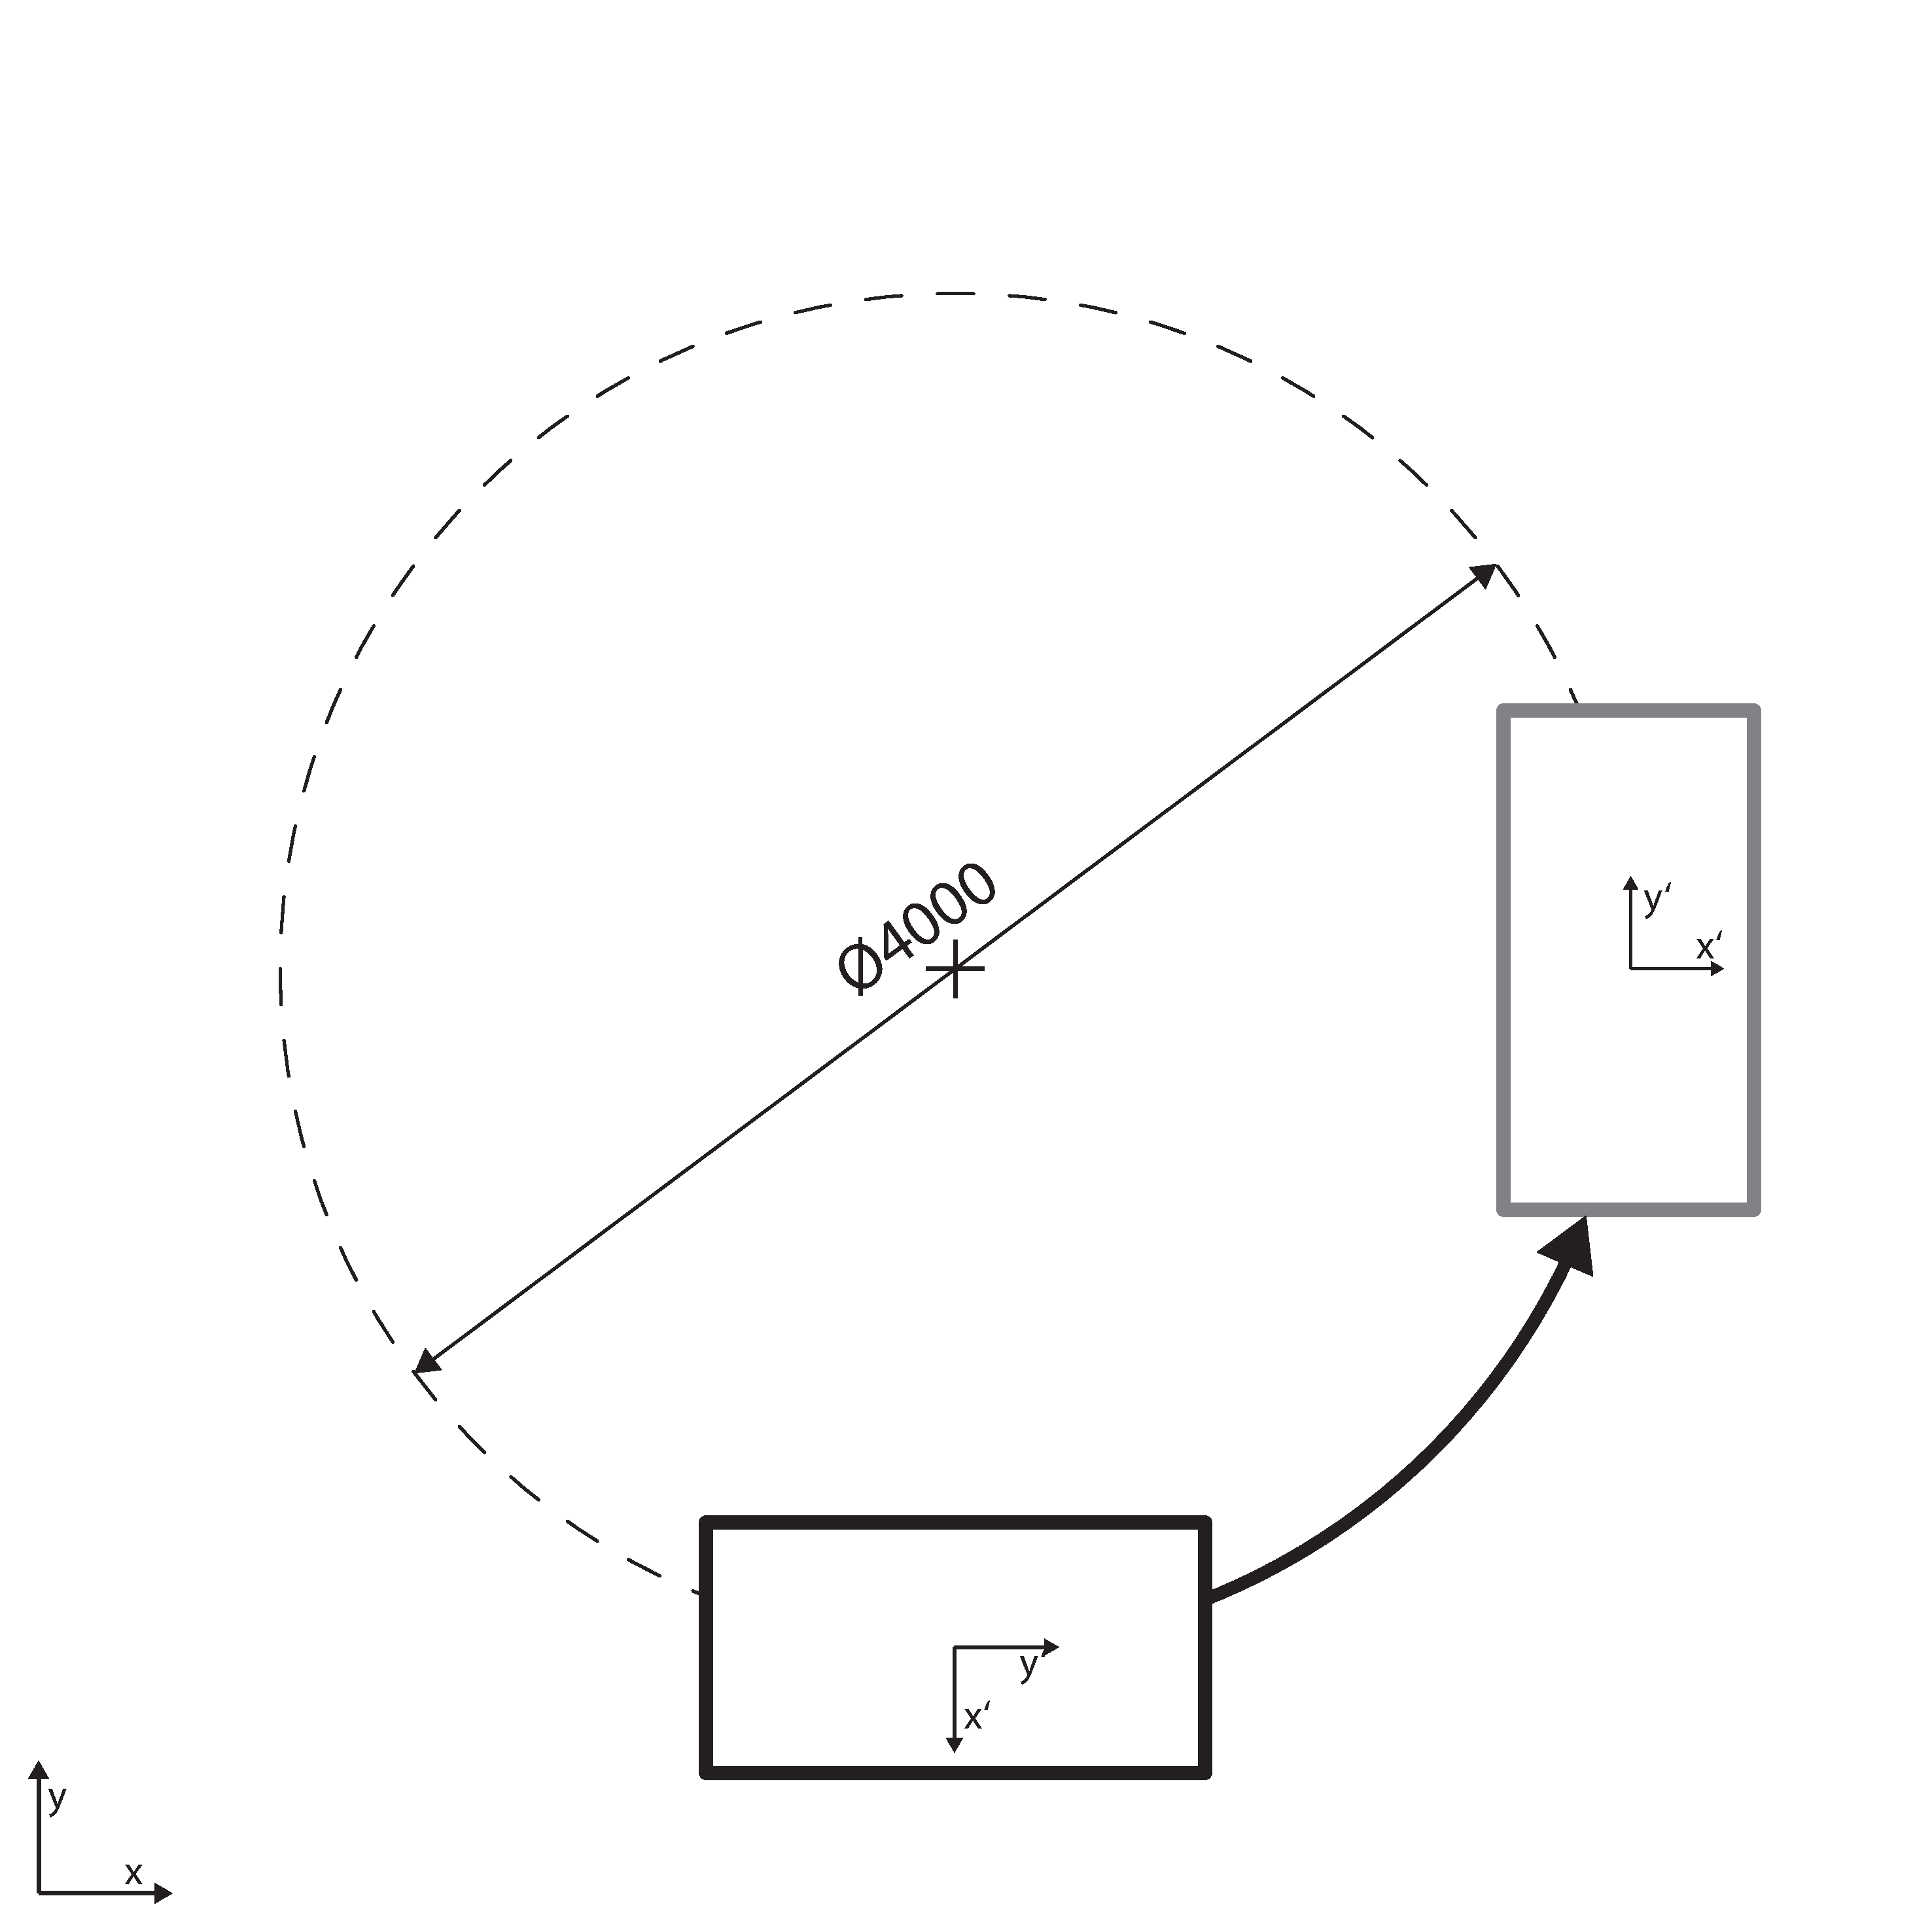
\includegraphics[width=.6\textwidth]{Abbildungen/Viertelkreis-vorwaerts}
    \caption{Kreisfahrt vorwärts}
    \label{fig:kreis-vorwaerts}
\end{figure}
Der Mecanum-Roboter fährt einen normalen Viertelkreis. Das Koordinatensystem des Roboters dreht sich dabei während der Kreisfahrt mit, $y'$ ist Tangente an den gefahrenen Kreis.

\begin{figure}[H]
    \centering
    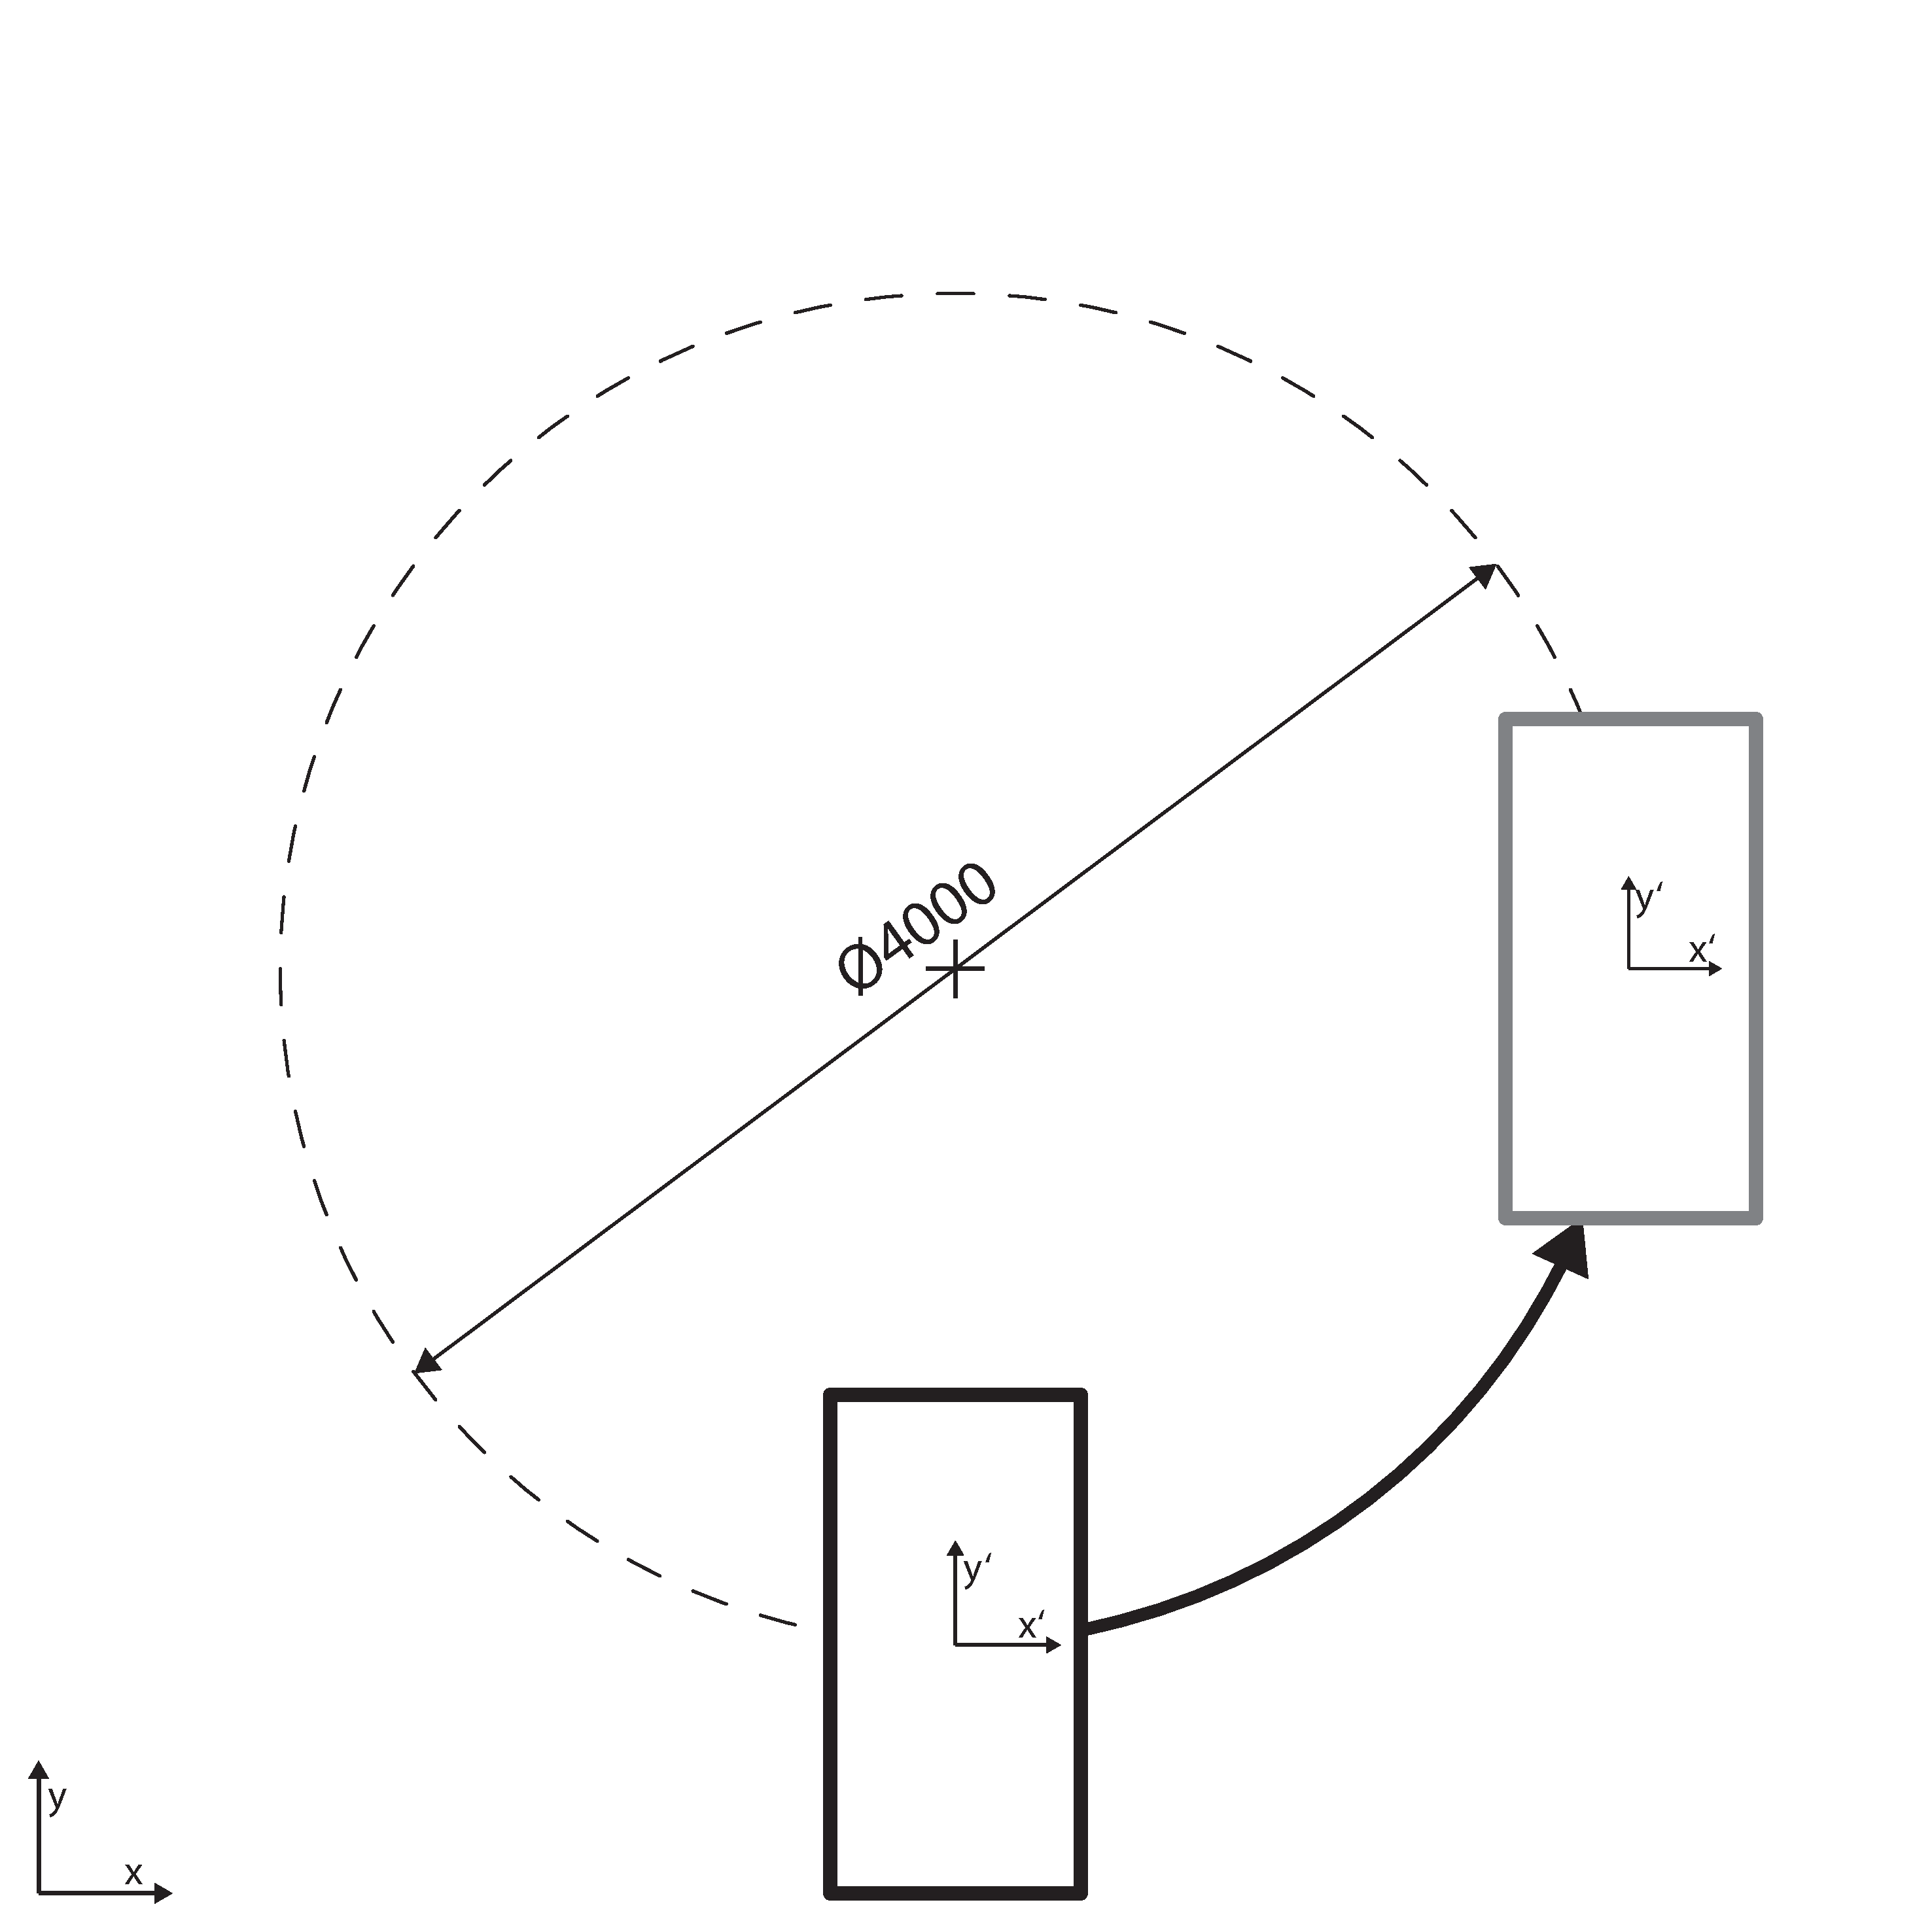
\includegraphics[width=.6\textwidth]{Abbildungen/Viertelkreis-translatorisch}
    \caption{Translatorische Kreisfahrt}
    \label{fig:kreis-translatorisch}
\end{figure}
Das Koordinatensystem des Roboters ist stets parallel zu den Raumkoordinaten während der Robotermittelpunkt im Raum einen Kreis abfährt.

\begin{figure}[H]
    \centering
    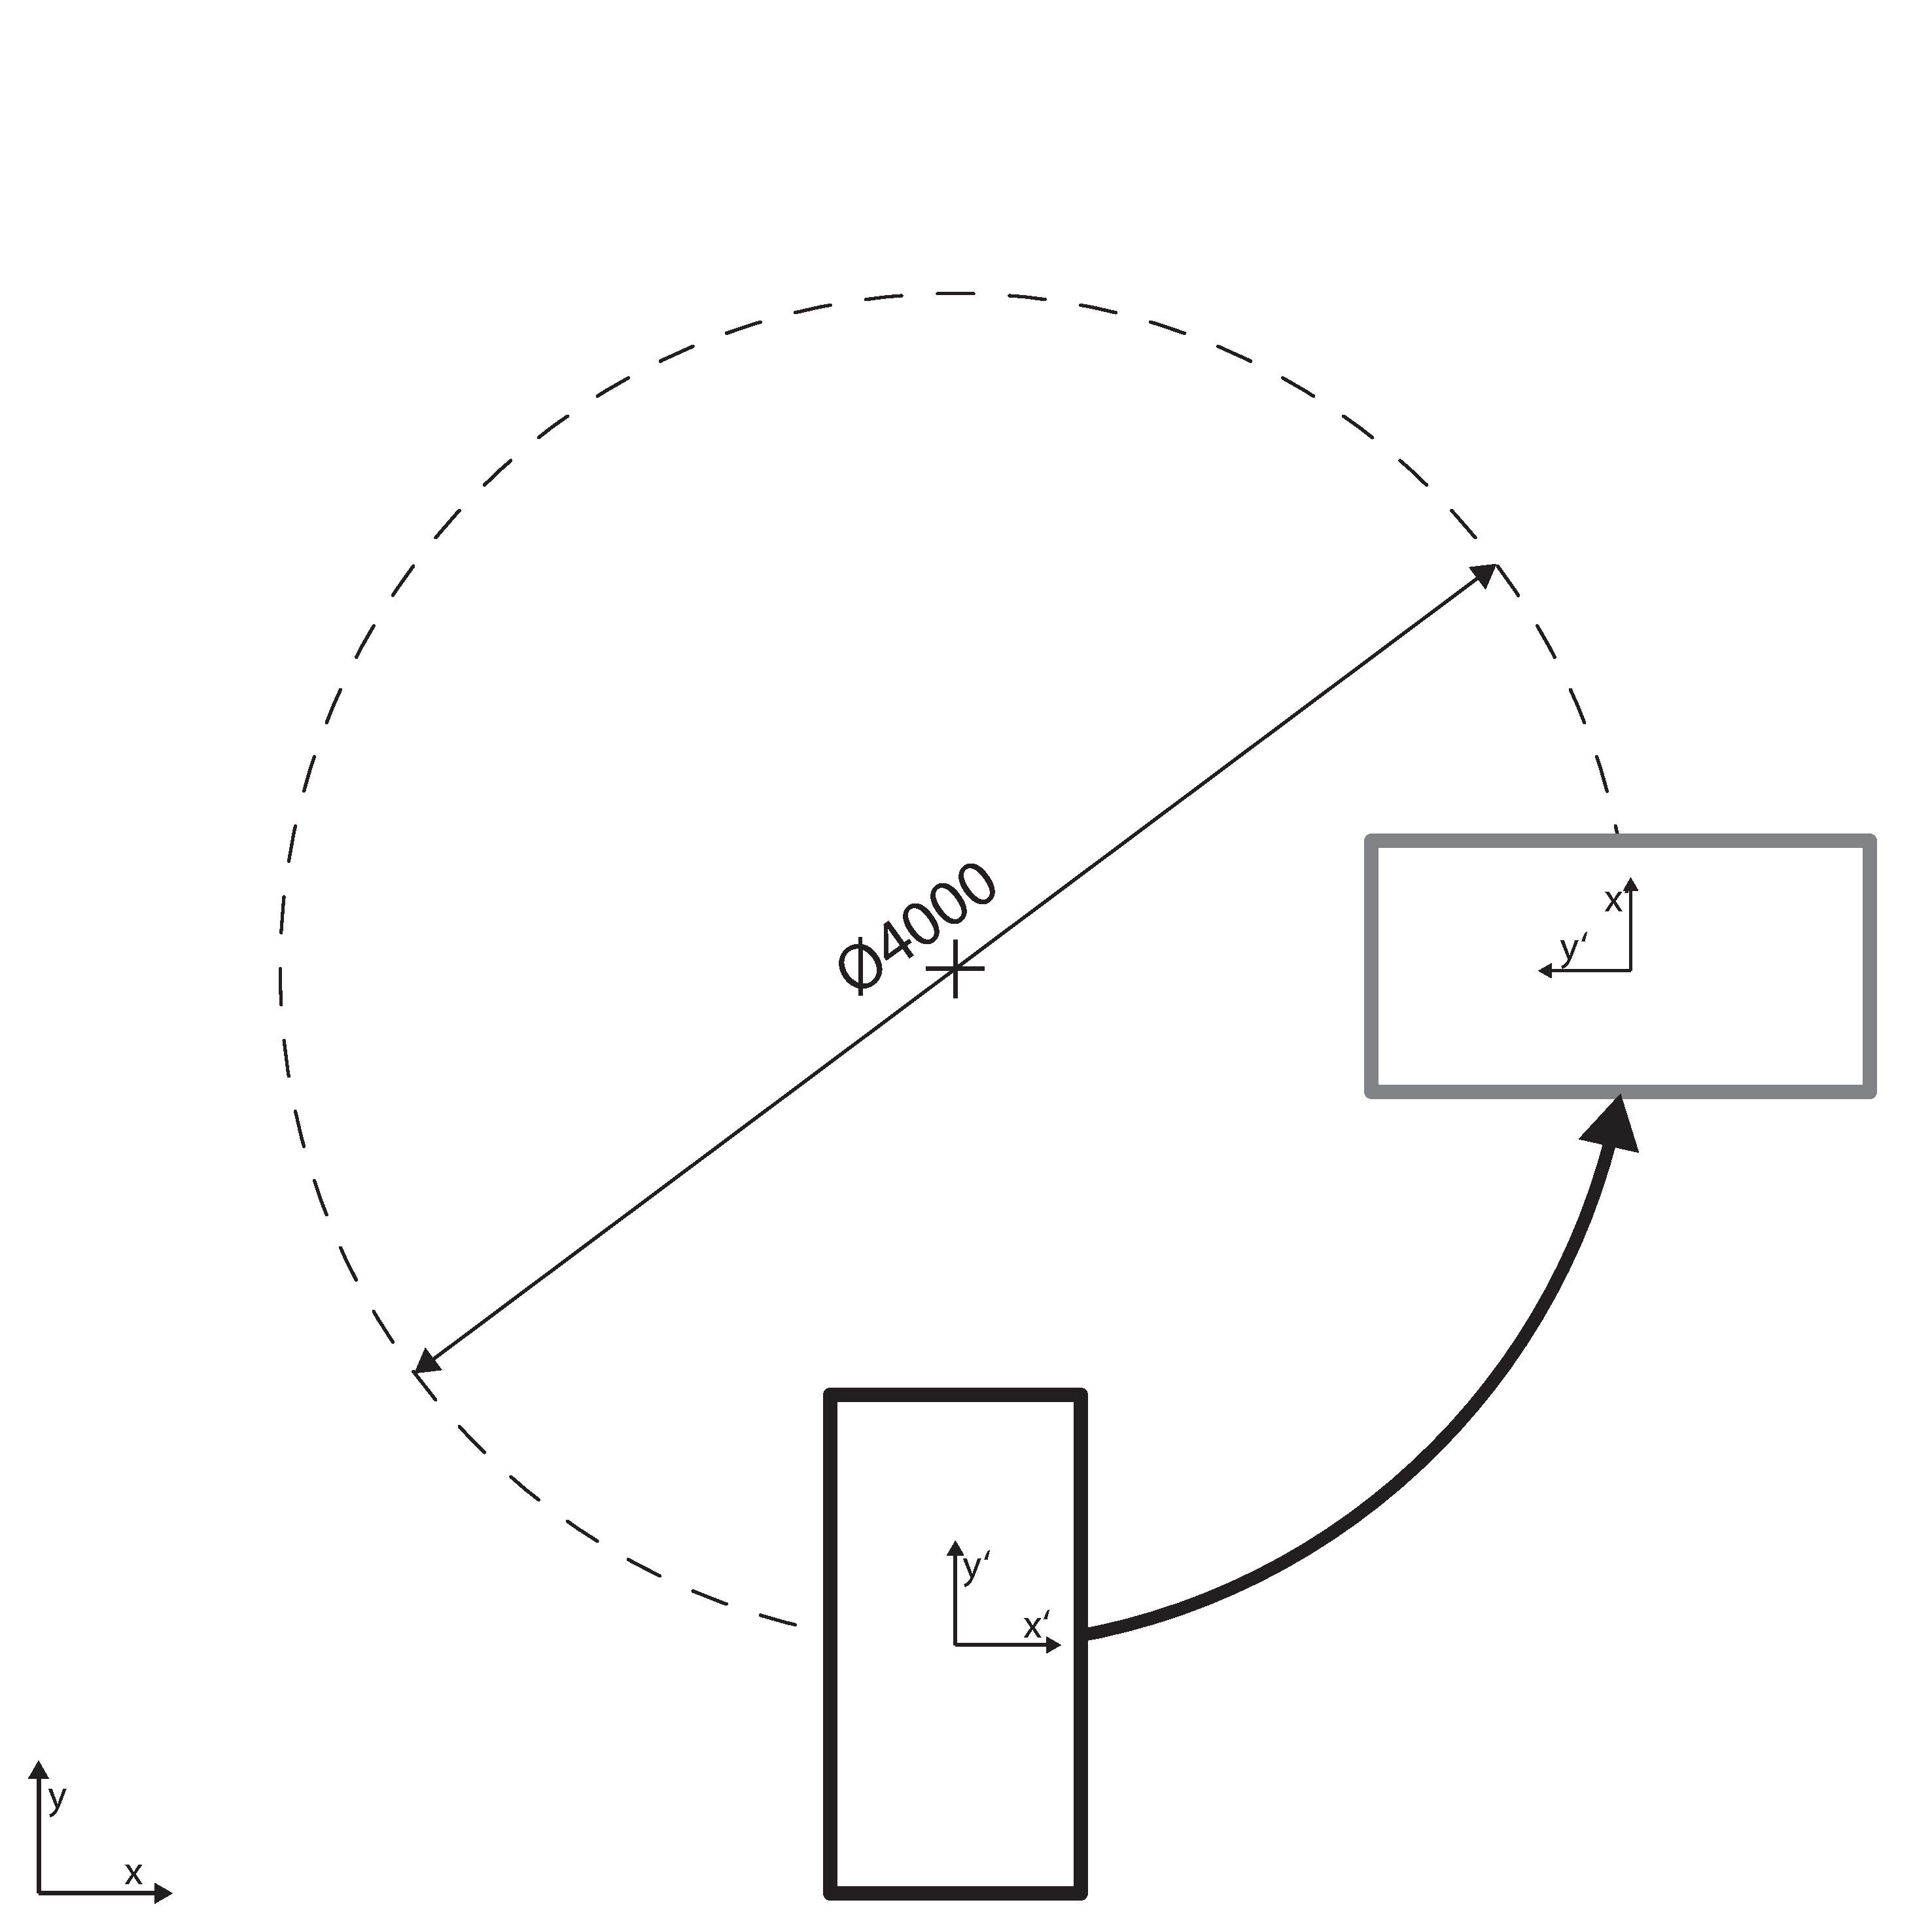
\includegraphics[width=.6\textwidth]{Abbildungen/Viertelkreis-seitwaerts}
    \caption{Kreisfahrt seitlich}
    \label{fig:kreis-seitwaerts}
\end{figure}
Das Koordinatensystem des Roboters gegenüber Abbildung~\ref{fig:kreis-vorwaerts} um $90^\circ$ gedreht. $x'$ ist Tangente an den gefahrenen Kreis.
